\chapter{Artificial Neural Network}

\subsection*{Formulas}

\textbf{Activation functions:}\\[0.5em]
\begin{tabular}{ll}
   Step function: & $f(x) = \begin{cases} 1 & \text{if } x \geq 0 \\ 0 & \text{if } x < 0 \end{cases}$ \\[0.5em]
   Sigmoid function: & $f(x) = \frac{1}{1 + e^{-x}}$ \\[0.5em]
   Tanh function: & $f(x) = \frac{e^x - e^{-x}}{e^x + e^{-x}}$ \\[0.5em]
   ReLU function: & $f(x) = \max(0, x)$ \\[0.5em]
\end{tabular}


\begin{tabular}{ll}
   Output &: $y_p = \sigma\left(\sum w_i x_i - \theta\right)$ \\
   Error &: $e = y_t - y_p$ \\
   Error gradient (output layer) &: $\delta = y \cdot [1-y] \cdot e$ \\
   Error gradient (hidden layer) &: $\delta_i = y_i \cdot [1-y_i] \cdot \sum \delta_j w_{ij}$ \\
   Weight update &: $w_{ij}' = w_{ij} + \alpha \delta_j y_i$ \\
\end{tabular}



\vspace{1em}
\textbf{Question:} For the following perceptron, the feature vector is $X$ = [1  0  1] and the desired output is $Y=1$. Consider the threshold value $\theta = 0.3$, learning rate $\alpha = 0.1$, initial weights $W_1 = 0.3$, $W_2 = 0.5$, and $W_3 = 0.6$.
i) Measure the predicted output and
ii) Calculate the updated weights (Wi, Wz and W3) after one iteration.


\textbf{Solution:} \\[0.5em]
For $P=1$,\\[0.5em]
$\begin{aligned}
   Y' &= \text{Step}(\left[(W1*X1 + W2*X2 + W3*X3) - \theta\right])\\[0.5em]
   & = \text{Step}(0.3 \times 1 + 0.5 \times 0 + 0.6 \times 1) - 0.3 = 0.6 \\
   & = \text{Step}(0.6) = 1
\end{aligned}$

$\therefore$ Error $E = Y - Y' = 1 - 1 = 0$

Since there is no error, no weight update is needed.

\textbf{Weight update:}\\[0.5em]
$\begin{aligned}
   & w_1' &= w_1 + \alpha x_1 E = 0.3 + 0.1 \times 1 \times 0 = 0.3 \\
   & w_2' &= w_2 + \alpha x_2 E = 0.5 + 0.1 \times 0 \times 0 = 0.5 \\
   & w_3' &= w_3 + \alpha x_3 E = 0.6 + 0.1 \times 1 \times 0 = 0.6 \\
\end{aligned}$

\pagebreak
For the following back propagation neural network shown in Figure 2, the feature vector is $X$ = [1 1] and the desired output is $Y=0$. Consider the threshold value $\theta_1 = 0.5$, $\theta_2 = -1.5$, $\theta_3 = 1.5$, learning rate $\alpha = 0.5$, initial weights $W_1 = 1$, $W_2 = -0.5$, $W_3 = 1$, $W_4 = 1$, $W_5 = 1$, and $W_6 = 1$.
\begin{enumerate}
   \item Measure the predicted outputs of the hidden layer (neuron $h_1$ and $h_2$).
   \item Measure the predicted output of the output layer (neuron $o_1$).
   \item Calculate the updated weights of output layer ($W_5$ and $W_6$) after one iteration.
\end{enumerate}

\begin{figure}[H]
   \centering
   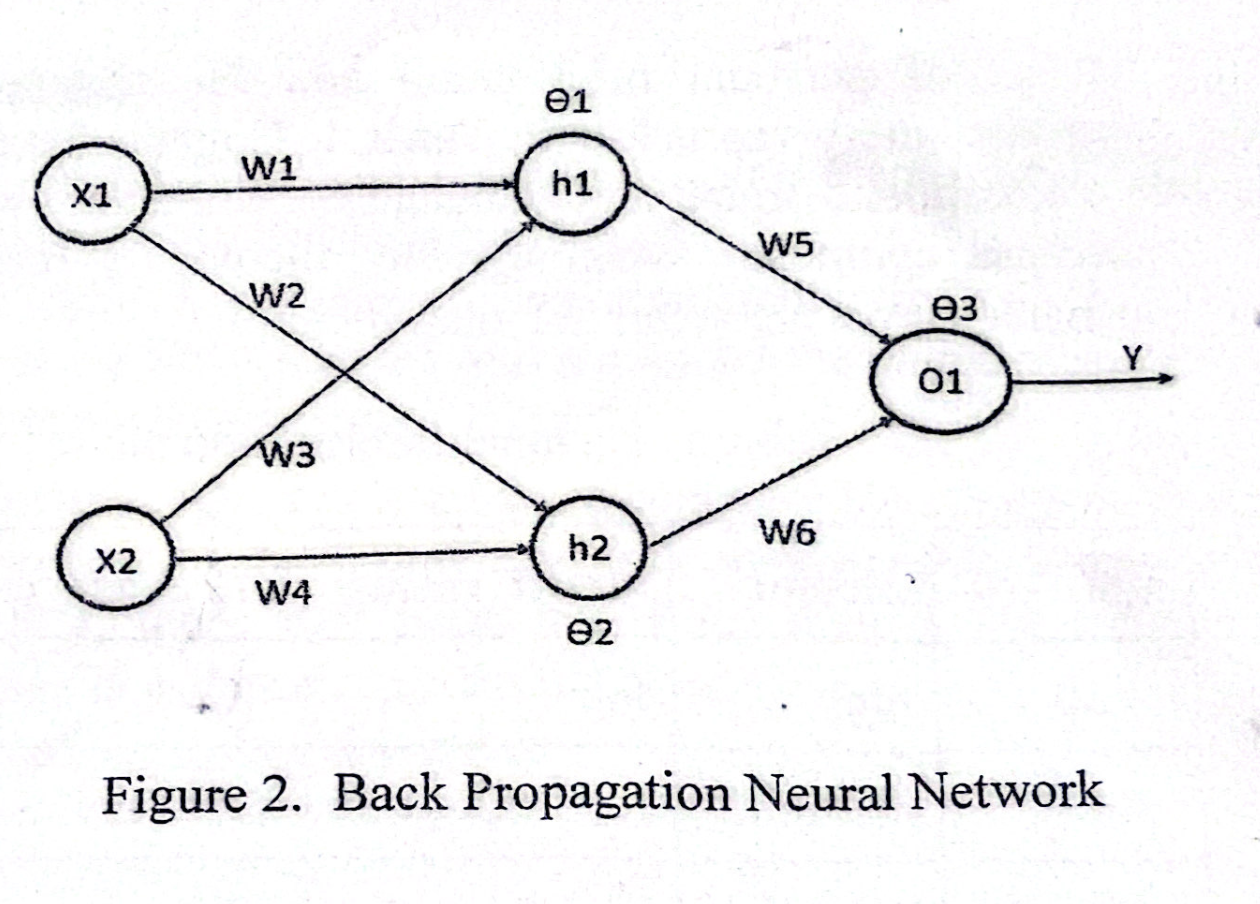
\includegraphics[width=0.5\textwidth]{figures/BPNN_Fall24.png}
\end{figure}

\textbf{Solution:} \\[0.5em]
\textbf{For hidden layer:}\\[0.5em]
$\begin{aligned}
   Y_{h_1} &= \sigma\left[(W_1 X_1 + W_3 X_2) - \theta_1\right] = \sigma\left[(1 \times 1 + 1 \times 1) - 0.5\right] = \sigma(1.5) = \frac{1}{1+e^{-1.5}} = 0.8176 \\
   Y_{h_2} &= \sigma\left[(W_2 X_1 + W_4 X_2) - \theta_2\right] = \sigma\left[(-0.5 \times 1 + 1 \times 1) - (-1.5)\right] = \sigma(2) = \frac{1}{1+e^{-2}} = 0.8807
\end{aligned}$
\vspace{0.5em}

\textbf{For output layer:}\\[0.5em]
$\begin{aligned}
   Y_{o1} &= \sigma\left[(W_5 Y_{h_1} + W_6 Y_{h_2}) - \theta_3\right] = \sigma\left[(1 \times 0.8176 + 1 \times 0.8807) - 1.5\right]  = \sigma(0.1983) = 0.5494
\end{aligned}$
\vspace{0.5em}

Now calculating error at output level,\\[0.5em]
$E_{o1} = Y - Y_{01} = 0 - 0.5494 = -0.5494$


Now calculating error gradient,\\[0.5em]
$\delta_{o1} = Y_{o1} \cdot [1-Y_{o1}] \cdot E_{o1} = 0.5494 \cdot [1-0.5494] \cdot (-0.5494) = -0.136$

Now updating weight between output and hidden layer,\\[0.5em]
$\begin{aligned}
   W_5' &= W_5 + \alpha Y_{o1} \delta_{o1} = 1 + 0.5 \times 0.5494 \times -0.136 = 0.96 \\
   W_6' &= W_6 + \alpha Y_{o1} \delta_{o1} = 1 + 0.5 \times 0.5494 \times -0.136 = 0.96
\end{aligned}$

Error gradients at hidden layer,\\[0.5em]
$\begin{aligned}
   \delta_{h1} &= Y_{h1} \cdot [1-Y_{h1}] \cdot \left[W_5\delta_{o1}\right]
   = 0.8176 \cdot [1-0.8176] \cdot \left[1 \times -0.136\right] = -0.02 \\
   \delta_{h2} &= Y_{h2} \cdot [1-Y_{h2}] \cdot \left[W_6\delta_{o1}\right]
   = 0.8807 \cdot [1-0.8807] \cdot \left[1 \times -0.136\right] = -0.01
\end{aligned}$

Now updating weight between hidden and input layer,\\[0.5em]
$\begin{aligned}
   W_1' &= W_1 + \alpha X_1 \delta_{h1} = 1 + 0.5 \times 1 \times -0.02 = 0.99 \\
   W_2' &= W_2 + \alpha X_2 \delta_{h2} = -0.5 + 0.5 \times 1 \times -0.02 = -0.51 \\
   W_3' &= W_3 + \alpha X_1 \delta_{h1} = 1 + 0.5 \times 1 \times -0.01 = 0.995 \\
   W_4' &= W_4 + \alpha X_2 \delta_{h2} = 1 + 0.5 \times 1 \times -0.01 = 0.995
\end{aligned}$